\section{Introduction}

The previous chapter established the importance of choosing the correct medium and metaphor for the understanding of complex datasets. For relational data exploring the relationship between any set of items, the sociograph style of representation was found to be the most effective. This chapter builds on that analogy and explores how this may be further improved. I start with looking at the current use of sociograms within chemistry (\autoref{sec:chemgraph}), the methods in which these can be made more useful (\autoref{syntatic},\autoref{semantic}), and finally apply this to a case study representing the atmospheric chemistry within the city of Beijing, China (\autoref{sec:chemcase}).

\subsection{Networks and their role within Visual Analytics (VA)} \label{sec:va}
Networks are present everywhere - This ranges from interactions within social media to bank transactions, internet routing, animal migration (nature paper with good vis), epidemiology, transport, everywhere... \cite{worldmap,a,b,c}. This is because the sociogram (or graph) structure may be applied to any set of items which contain one or more relationships between them. With academia, networks have been invaluable to the field of gene-activation and metabolic pathways (Biology);\textit{EXAMPLE FIX: suspects and organised crime / terrorist cells (secret service or police) and the complex networks of relationships between system components and users (software engineering) \cite{IPSEPCOLA} }. Within the information visualisation field (InfoVis), items are referred to as nodes, or vertices, and their relationships are called edges, or links \cite{ch1}. These terms can be used interchangeably and will do, throughout this thesis. 


\subsection{Graphs in Chemistry}\label{sec:chemgraph}



Node link representations have been a core part of the field of chemistry for many years. They are integral in the representation of molecules, using the ball-stick (graph) style analogy, both physically (with the aid of molecular model kits) or pictorially to show various structural properties, \autoref{fig:mol}. Using such analogies aid in the tasks of identifying the features, functional groups and bond properties of the species and how they can react.  

\begin{figure}[H]
    \centering
    \begin{subfigure}[b]{0.24\textwidth}
        \centering
        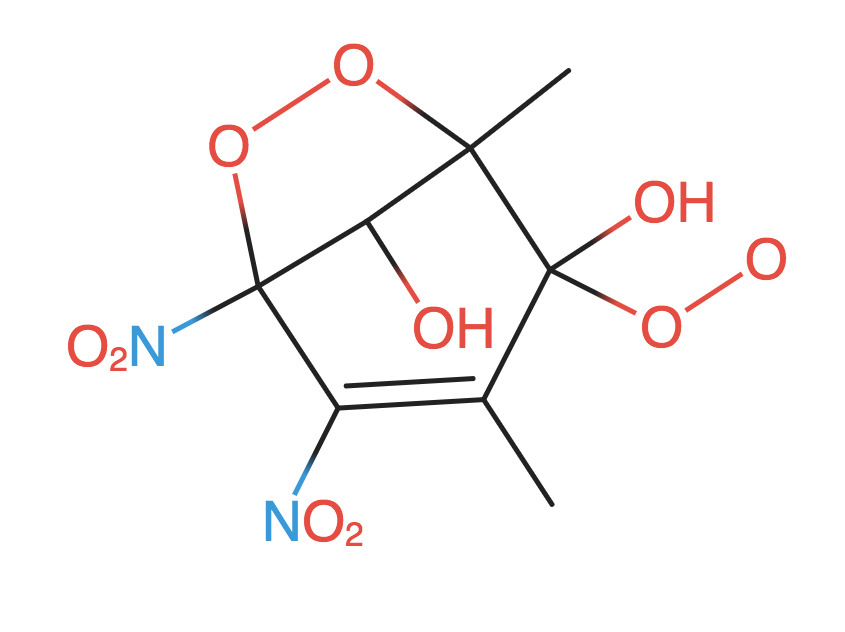
\includegraphics[width=\textwidth]{figures_c1/mol2d.png}
        \caption{2D `classic'\\ representation}
    \end{subfigure}
    \begin{subfigure}[b]{0.235\textwidth}
        \centering
        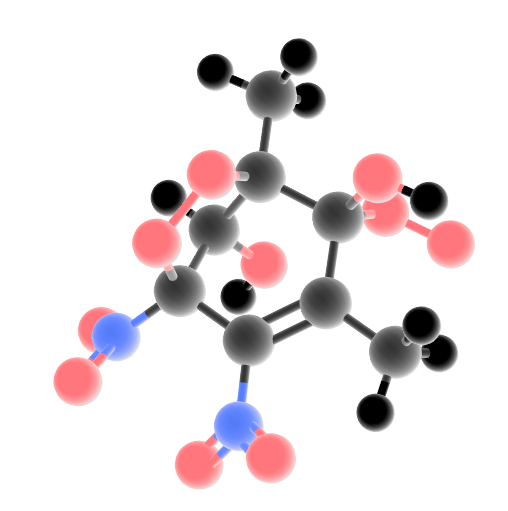
\includegraphics[width=\textwidth]{figures_c1/mol3d.png}
        \caption{3D representation}
    \end{subfigure}
       \caption{\textbf{An example molecule represented in two and three dimensions.} These have been created  using the SmilesJS and Mol3D software, \cite{smiles, mol3d} }
       \label{fig:mol}
\end{figure}

Within the master chemical mechanism (MCM) \cite{mcm}, referenced in \autoref{sec:dataset}, we see such properties used used to determine the reaction pathways species may undergo \autoref{fig:protocol}. In mechanistic development, the degradation of larger species is represented as a series of interconnected reactions in the form of a reaction cycle, \autoref{fig:butane}. Such patterns often have to be manually simplified to best represent the chemistry of the system. 

\begin{figure}[H]
    \centering
        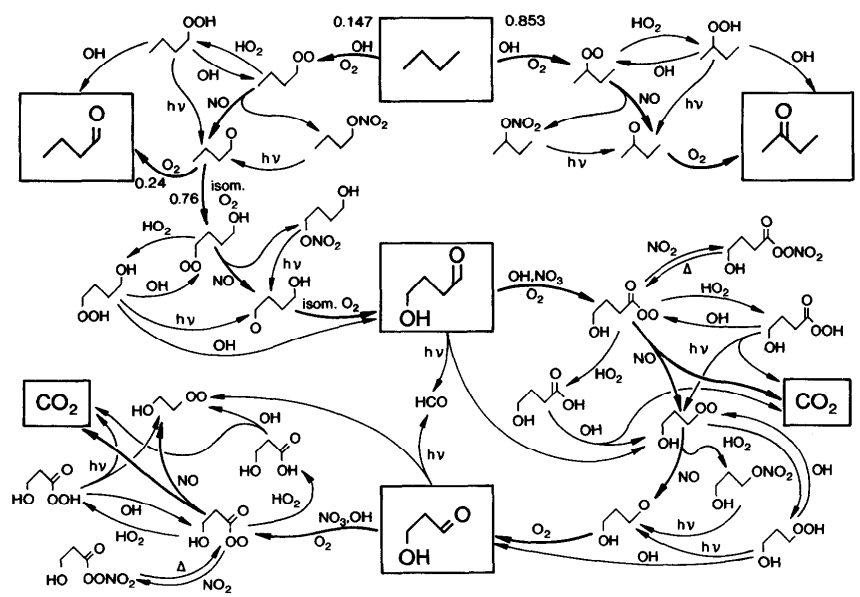
\includegraphics[width=\textwidth]{figures_c1/butane.png}

       \caption{\textbf{A systematic representation of the degregation of butane.} Source: \cite{butane} }
       \label{fig:butane}
\end{figure}

This type of sociograph has many similarities with a simple directed graph. Links are representative of the direction of reaction and show the relationships between different species (the nodes). The main difference between this and a conventional graph is that species have been duplicated to aid clarity, a feature which will not occur with the core mechanism, and consequently any mathematical graph which may be generated from it. The flow-like nature makes this type of representation makes it easier to understand as a human, than any list of reactions could ever be. The reason for this lies in a combination of evolutionary traits, whereupon we are genetically predispositioned to comprehend patterns and intemperate shapes faster than written characters. 


\subsection{Modeling chemistry as a directed graph.}

Historically it is seen that the graph format has proven to be an efficient means of understanding the reactions within a mechanism. Traditionally these are constructed manually, with the designer making a series of choices on how best to place, and simplify the chemistry based on their application. As our understanding of chemistry improves and we begin to progress into automated and semi-automated mechanism construction. This makes the construction of mechanisms with tens of millions of species and billions of reaction possible. It is at this point where the manual design and simplification of reaction networks becomes infeasible. 

Today automatic graph layouts allow us to generate multivariate and complex graphs easily. This means that, much like in the construction of a mechanism, we can rely on computer-aided design to generate a directed graph representation of the chemistry. \cite{sciamerican} states that "The beauty of a good information graphic is that it can tell a whole story in a single unit of visual content". This is particularly true for the use of directed graphs in chemistry where we can compare different mechanism subsets,(\autoref{fig:meccomp}) or model simulations (\autoref{sec:diurnal}).

However, as with everything several problems emerge from the complete automation of a task. Firstly real-world data very rarely reacts how it is expected to. Here networks of high edge density often obfuscate the graph data, and produce what is only described as a `birds nest', `hairball' or `ball of yarn' within the literature, \cite{ch7}. Although such disasters and mishaps can be seen as moments of turbulence, they encourage a greater understanding of the design process and can catalyze to merge dissimilar ideas into an effective visualisation \cite{goodideas}. 



\begin{figure}[H]
     \centering
     \begin{subfigure}[b]{0.29\textwidth}
         \centering
         % \includegraphics[width=\textwidth]{figures_c1/}
         \caption{Full MCM}
     \end{subfigure}
     \begin{subfigure}[b]{0.29\textwidth}
         \centering
         % \includegraphics[width=\textwidth]{figures_c1/}
         \caption{Borneo}
     \end{subfigure}
     \begin{subfigure}[b]{0.29\textwidth}
         \centering
         % \includegraphics[width=\textwidth]{figures_c1/}
         \caption{London}
     \end{subfigure}
        \caption{\textbf{Looking at mechanism subsets using subgraphs. } We compare how the mechanism subsets used to model chemistry within two different environments vary. These are Borneo, red.... and show the ...   }
        \label{fig:mechcomp}
\end{figure}





% “In fast-paced settings, it is important to know if the visualization is going to be so complex that the signals may be obscured,” explained Eugene Wu, an assistant professor of computer science and co-author of a paper on this method. For instance, 


%in high-stakes medical settings, such as when physicians are reading EEGs in emergency rooms, the most important information needs to stand out quickly in a visualization, which can be obscured by a static of unnecessary data.

% Such developments could further empower scientists to discover trends and patterns in their data.

% ILLUSTRATIONS THAT HELP US UNDERSTAND SCIENCE
% Visualizing large quantities of complex information in an elegantly simple way is no easy task. That’s why Killer differentiates visual communication from design: the former is a specialized skill that involves juggling both form and function, so that you create something that’s not only beautiful, but meaningful as well.



% \\\\\

% The beauty of a good information graphic is that it can tell a whole story in a single unit of visual content. As much as I’ve come to roll my eyes at the overused headline format, “[Such and Such Concept] Explained in One Graphic,” this convention does capture the strength of the graphic as a medium. (The headline certainly becomes less compelling when revised to read, “[Such and Such Concept] Explained in Several Paragraphs.”) Because while information graphics often do require their audience to do some reading, the text tends to be broken up into manageable chunks and arranged for easy consumption together with visual elements. 

% There is also something about an information graphic that inspires trust in its content; seeing a concept visualized gives it a certain amount of objective weight. Surely this idea can be used to ignoble ends, as seen in certain deliberately deceptive data visualizations. But more often than not, I believe it is harder to lie with a graphic than it is with words alone—if only because it requires much more effort to visualize something for which there exists no factual reference. 

% https://blogs.scientificamerican.com/sa-visual/how-science-visualization-can-help-save-the-world/
